\section{Hiện thực dự án}

\subsection{Kết nối phần cứng}
Vi điều khiển STM32F103RB trên kit XNUCLEO-F103RB được cấu hình giao tiếp với các linh kiện ngoại vi thông qua các chân Header chuẩn Arduino Uno. Bảng~\ref{tab:hardware_pinout} trình bày chi tiết sơ đồ gán chân thực tế trong dự án:

\begin{table}[!htbp]
\centering
\footnotesize
\setlength{\tabcolsep}{3.5pt}
\renewcommand{\arraystretch}{1.25}
\begin{tabularx}{\textwidth}{|>{\raggedright\arraybackslash}X|>{\centering\arraybackslash}p{1.4cm}|>{\centering\arraybackslash}p{1.9cm}|>{\raggedright\arraybackslash}p{2.5cm}|>{\raggedright\arraybackslash}p{2.7cm}|}
\hline
\textbf{Thiết bị / Module} & \textbf{Chân Arduino} & \textbf{Chân STM32} & \textbf{Chế độ GPIO} & \textbf{Tên nhãn (User Label)} \\ \hline
Đèn giao thông 1 (Tín hiệu A) & D3 & PB3 & Output Push-Pull & \texttt{TL1\_A} \\ \hline
Đèn giao thông 1 (Tín hiệu B) & D4 & PB5 & Output Push-Pull & \texttt{TL1\_B} \\ \hline
Đèn giao thông 2 (Tín hiệu A) & D5 & PB4 & Output Push-Pull & \texttt{TL2\_A} \\ \hline
Đèn giao thông 2 (Tín hiệu B) & D6 & PB10 & Output Push-Pull & \texttt{TL2\_B} \\ \hline
Nút nhấn 1 (Chuyển chế độ) & D7 & PA8 & Input Pull-up & \texttt{BTN\_1} \\ \hline
Nút nhấn 2 (Action / Chọn trường) & D8 & PA9 & Input Pull-up & \texttt{BTN\_2} \\ \hline
Nút nhấn 3 (Giảm giá trị) & D9 & PC7 & Input Pull-up & \texttt{BTN\_3} \\ \hline
Nút nhấn 4 (Tăng giá trị) & D10 & PB6 & Input Pull-up & \texttt{BTN\_4} \\ \hline
LED trạng thái hệ thống & -- & PA5 & Output Push-Pull & \texttt{LD2 [Green Led]} \\ \hline
Nút nhấn USER trên mạch & -- & PC13 & Input Floating & \texttt{B1 [Blue PushButton]} \\ \hline
Cảm biến DHT20 \& LCD (I2C1) & Khe I2C & PB8 (SCL), PB9 (SDA) & I2C Alternate Function & I2C1 (0x38, 0x27) \\ \hline
\end{tabularx}
\caption{Bảng ánh xạ kết nối chân phần cứng của hệ thống}
\label{tab:hardware_pinout}
\end{table}

Mỗi module đèn giao thông sử dụng 2 đường điều khiển tín hiệu số để hiển thị 4 trạng thái đèn (Tắt, Đỏ, Vàng, Xanh). Kết quả đo đạc thực tế trên mạch được tổng hợp trong Bảng~\ref{tab:traffic_truth_table}:

\begin{table}[H]
\centering
\begin{tabular}{|c|c|c|l|}
\hline
\textbf{Tín hiệu 1 (Pin A)} & \textbf{Tín hiệu 2 (Pin B)} & \textbf{Trạng thái đèn} & \textbf{Mô tả} \\ \hline
\texttt{0} & \texttt{0} & \textbf{Tắt (\texttt{TL\_OFF})} & Cả 3 đèn đều tắt \\ \hline
\texttt{0} & \texttt{1} & \textbf{Vàng (\texttt{TL\_AMBER})} & Đèn màu Vàng sáng \\ \hline
\texttt{1} & \texttt{0} & \textbf{Xanh (\texttt{TL\_GREEN})} & Đèn màu Xanh sáng \\ \hline
\texttt{1} & \texttt{1} & \textbf{Đỏ (\texttt{TL\_RED})} & Đèn màu Đỏ sáng \\ \hline
\end{tabular}
\caption{Bảng chân trị tín hiệu điều khiển module đèn giao thông}
\label{tab:traffic_truth_table}
\end{table}

Đoạn mã cấu hình chân GPIO được sinh từ STM32CubeIDE trong hàm \texttt{MX\_GPIO\_Init()} như sau:
\begin{lstlisting}[language=C, caption={Trích đoạn cấu hình GPIO trong file main.c}]
static void MX_GPIO_Init(void) {
  GPIO_InitTypeDef GPIO_InitStruct = {0};

  /* Bat clock cac ngoai vi GPIO */
  __HAL_RCC_GPIOC_CLK_ENABLE();
  __HAL_RCC_GPIOA_CLK_ENABLE();
  __HAL_RCC_GPIOB_CLK_ENABLE();

  /* Muc logic mac dinh cho cac chan Output den giao thong */
  HAL_GPIO_WritePin(GPIOA, LD2_Pin, GPIO_PIN_RESET);
  HAL_GPIO_WritePin(GPIOB, TL1_A_Pin|TL2_A_Pin|TL1_B_Pin|TL2_B_Pin, GPIO_PIN_RESET);

  /* Cau hinh chan Nhan nut B1 tren kit */
  GPIO_InitStruct.Pin = B1_Pin;
  GPIO_InitStruct.Mode = GPIO_MODE_IT_RISING;
  GPIO_InitStruct.Pull = GPIO_NOPULL;
  HAL_GPIO_Init(B1_GPIO_Port, &GPIO_InitStruct);

  /* Cau hinh Output cho cac chan den giao thong PB3, PB4, PB5, PB10 */
  GPIO_InitStruct.Pin = TL1_A_Pin|TL2_A_Pin|TL1_B_Pin|TL2_B_Pin;
  GPIO_InitStruct.Mode = GPIO_MODE_OUTPUT_PP;
  GPIO_InitStruct.Pull = GPIO_NOPULL;
  GPIO_InitStruct.Speed = GPIO_SPEED_FREQ_LOW;
  HAL_GPIO_Init(GPIOB, &GPIO_InitStruct);

  /* Cau hinh Input Pull-up cho cac nut nhan BTN_1, BTN_2 */
  GPIO_InitStruct.Pin = BTN_1_Pin|BTN_2_Pin;
  GPIO_InitStruct.Mode = GPIO_MODE_INPUT;
  GPIO_InitStruct.Pull = GPIO_PULLUP;
  HAL_GPIO_Init(GPIOA, &GPIO_InitStruct);

  /* Cau hinh BTN_3 (PC7) va BTN_4 (PB6) */
  GPIO_InitStruct.Pin = BTN_3_Pin;
  HAL_GPIO_Init(BTN_3_GPIO_Port, &GPIO_InitStruct);
  GPIO_InitStruct.Pin = BTN_4_Pin;
  HAL_GPIO_Init(BTN_4_GPIO_Port, &GPIO_InitStruct);
}
\end{lstlisting}

\subsection{Hiện thực scheduler}

\subsubsection{Lựa chọn cấu trúc dữ liệu và cơ chế Delay tương đối đạt $\mathcal{O}(1)$}

\textbf{So sánh mảng tĩnh (Array) và danh sách liên kết (Linked List)}
Trong thiết kế hệ thống nhúng thời gian thực trên vi điều khiển có tài nguyên bộ nhớ giới hạn như STM32F103RB (20~KB SRAM, 128~KB Flash), việc lựa chọn cấu trúc dữ liệu quản lý tác vụ đóng vai trò then chốt:
\begin{itemize}
    \item \textbf{Danh sách liên kết (Linked List)}: 
    \begin{itemize}
        \item \textit{Ưu điểm}: Việc chèn và xóa nút diễn ra linh hoạt, độ phức tạp thao tác con trỏ cục bộ là $\mathcal{O}(1)$ khi đã xác định vị trí.
        \item \textit{Nhược điểm}: Cần cấp phát và giải phóng động (\texttt{malloc}/\texttt{free}), tiềm ẩn nguy cơ phân mảnh bộ nhớ SRAM nghiêm trọng sau thời gian dài vận hành, có thể dẫn đến treo vi điều khiển (Crash/HardFault). Ngoài ra, mỗi node tốn thêm 4 bytes con trỏ và dữ liệu nằm rải rác trong bộ nhớ làm giảm hiệu năng truy xuất do không tận dụng được cơ chế nạp trước ô nhớ liền kề.
    \end{itemize}
    \item \textbf{Mảng tĩnh (Array)}:
    \begin{itemize}
        \item \textit{Ưu điểm}: Bộ nhớ được cấp phát cố định một lần duy nhất tại vùng nhớ \texttt{.bss} ngay khi biên dịch (\texttt{SCH\_MAX\_TASKS = 40}), đảm bảo tính dự đoán được (deterministic) và an toàn tuyệt đối về mặt bộ nhớ. Các phần tử nằm liên tiếp trong RAM giúp vi điều khiển truy xuất cực nhanh.
        \item \textit{Nhược điểm}: Thao tác chèn hoặc xóa phần tử ở giữa mảng đòi hỏi dời các phần tử phía sau với độ phức tạp $\mathcal{O}(n)$. Tuy nhiên, thao tác thêm/xóa tác vụ chỉ diễn ra trong luồng nền (\texttt{SCH\_Add\_Task} lúc khởi tạo hoặc \texttt{SCH\_Dispatch\_Tasks} trong \texttt{while(1)}), hoàn toàn không ảnh hưởng đến tính thời gian thực của ngắt Timer ISR.
    \end{itemize}
\end{itemize}
Do đó, nhóm quyết định lựa chọn \textbf{Mảng tĩnh} kết hợp cấu trúc \texttt{sTask}:

\begin{lstlisting}[language=C, caption={Cấu trúc dữ liệu của một Task trong Scheduler}]
typedef struct {
    void (*pTask)(void); /* Con tro ham thuc thi task */
    uint32_t Delay;      /* So tick cho den lan chay ke tiep */
    uint32_t Period;     /* Chu ky lap lai tinh theo tick (0 neu la one-shot) */
    uint8_t  RunMe;      /* Co bao hieu task san sang chay */
    uint32_t TaskID;     /* Dinh danh duy nhat cua task */
} sTask;
\end{lstlisting}

\textbf{Giải thích cơ chế tổ chức danh sách theo Delay tương đối (Delta List)}

\textbf{a) Hạn chế của phương pháp độ trễ tuyệt đối (Absolute Delay -- $\mathcal{O}(n)$):}\\
Trong bộ định thời truyền thống, mỗi task khi đưa vào mảng lưu giữ trực tiếp số tick đếm lùi của chính nó. Mỗi khi có ngắt Timer (10ms tick), hàm \texttt{SCH\_Update()} bắt buộc phải duyệt qua toàn bộ $n$ tác vụ trong mảng. Khi số lượng tác vụ trong hệ thống tăng lên, thời gian chiếm dụng CPU trong chương trình phục vụ ngắt (ISR) tăng tuyến tính theo $\mathcal{O}(n)$, làm tăng độ trễ ngắt và có nguy cơ bỏ sót các sự kiện ngoại vi quan trọng khác.

\textbf{b) Nguyên lý tổ chức theo Độ trễ tương đối (Delta List):}\\
Để đưa thời gian xử lý trong ISR về hằng số $\mathcal{O}(1)$, danh sách tác vụ được tổ chức theo cấu trúc \textbf{Độ trễ tương đối (Relative Delay)}:
\begin{enumerate}
    \item Các task trong mảng \texttt{SCH\_tasks\_G} luôn được sắp xếp theo thứ tự thời gian hết hạn tăng dần từ trái sang phải:
    \begin{equation}
        T_0 \le T_1 \le T_2 \le \dots \le T_{n-1}
    \end{equation}
    với $T_k$ là tổng thời gian chờ tuyệt đối tính từ thời điểm hiện tại cho đến khi task $k$ được kích hoạt.
    \item Biến \texttt{Delay} của task đầu tiên lưu đúng thời gian chờ tuyệt đối của nó:
    \begin{equation}
        \text{Delay}_0 = T_0
    \end{equation}
    \item Biến \texttt{Delay} của các task tiếp theo ($i \ge 1$) \textbf{không lưu thời gian tuyệt đối}, mà chỉ lưu khoảng chênh lệch thời gian (Delta) so với task đứng ngay trước nó:
    \begin{equation}
        \text{Delay}_i = T_i - T_{i-1} \quad (i \ge 1)
    \end{equation}
    Ngược lại, thời điểm thực thi tuyệt đối $T_k$ của một task thứ $k$ bất kỳ chính là tổng tích lũy của tất cả các giá trị \texttt{Delay} từ đầu danh sách đến vị trí $k$:
    \begin{equation}
        T_k = \sum_{j=0}^{k} \text{Delay}_j
    \end{equation}
\end{enumerate}



\subsubsection{Hiện thực các hàm và giải thuật chi tiết}
Bảng~\ref{tab:scheduler_complexity} tổng hợp độ phức tạp thuật toán và vai trò của các hàm trong bộ định thời hợp tác:

\begin{table}[H]
\centering
\small
\setlength{\tabcolsep}{4pt}
\renewcommand{\arraystretch}{1.25}
\begin{tabularx}{\textwidth}{|l|c|>{\raggedright\arraybackslash}X|}
\hline
\textbf{Tên hàm} & \textbf{Độ phức tạp} & \textbf{Vai trò và giải thuật} \\ \hline
\texttt{SCH\_Init()} & $\mathcal{O}(n)$ & Xóa trắng danh sách tác vụ, đặt toàn bộ TaskID về 0 khi khởi động. \\ \hline
\texttt{SCH\_Update()} & $\mathcal{O}(1)$ & Gọi trực tiếp trong ngắt Timer 10ms. Cập nhật độ trễ của task đầu hàng đợi và bật cờ \texttt{RunMe}. \\ \hline
\texttt{SCH\_Add\_Task()} / \texttt{Insert()} & $\mathcal{O}(n)$ & Chèn task vào đúng vị trí theo độ trễ tương đối và cập nhật lại độ trễ của task liền sau. \\ \hline
\texttt{SCH\_Dispatch\_Tasks()} & $\mathcal{O}(n)$ & Gọi trong vòng lặp \texttt{while(1)} ở luồng nền. Thực thi task đến hạn, giải phóng One-shot task hoặc tái nạp task tuần hoàn. \\ \hline
\texttt{SCH\_Delete\_Task()} & $\mathcal{O}(n)$ & Tìm task theo ID, bù độ trễ cho task phía sau, giải phóng khe nhớ và dồn mảng. \\ \hline
\end{tabularx}
\caption{Độ phức tạp thuật toán của các hàm trong Scheduler}
\label{tab:scheduler_complexity}
\end{table}

Dưới đây là mã nguồn chi tiết và phân tích giải thuật của từng hàm trong file \texttt{scheduler.c}:

\paragraph{1. Hàm khởi tạo hệ thống -- \texttt{SCH\_Init()}}
\begin{lstlisting}[language=C, caption={Mã nguồn hàm SCH\_Init}]
void SCH_Init(void) {
  memset(SCH_tasks_G, 0, sizeof(SCH_tasks_G));
  SCH_count = 0;
  newTaskID = 0;
}
\end{lstlisting}

\textbf{Giải thích giải thuật}:
Hàm \texttt{SCH\_Init()} được gọi một lần duy nhất trong quá trình khởi động hệ thống. Hàm thực hiện xóa toàn bộ mảng tĩnh \texttt{SCH\_tasks\_G} bằng hàm \texttt{memset()}, thiết lập biến đếm số lượng tác vụ \texttt{SCH\_count = 0} và đặt lại bộ đếm định danh \texttt{newTaskID = 0}. Việc này đảm bảo không có rác bộ nhớ từ phiên chạy trước gây ra các hành vi không xác định.

\paragraph{2. Hàm cập nhật định thời trong ngắt Timer -- \texttt{SCH\_Update()}}
\begin{lstlisting}[language=C, caption={Mã nguồn hàm SCH\_Update}]
// Do phuc tap O(1)
void SCH_Update(void) {
  if (SCH_count == 0)
    return;
  if (SCH_tasks_G[0].Delay > 0)
    SCH_tasks_G[0].Delay--;
  if (SCH_tasks_G[0].Delay == 0)
    SCH_tasks_G[0].RunMe = 1;
}
\end{lstlisting}
\textbf{Giải thích giải thuật và chứng minh $\mathcal{O}(1)$}:
Hàm \texttt{SCH\_Update()} được đặt trong chương trình phục vụ ngắt (ISR) của Timer phần cứng (TIM2 chu kỳ 10ms).
\begin{itemize}
    \item Do danh sách tác vụ được tổ chức theo cấu trúc \textbf{Độ trễ tương đối}, toàn bộ thời gian trễ của các task phía sau đều phụ thuộc vào thời điểm hoàn thành của các task phía trước.
    \item Vì vậy, trong mỗi ngắt Timer (1 tick), vi điều khiển \textbf{chỉ cần kiểm tra và giảm duy nhất biến \texttt{Delay} của phần tử đứng đầu hàng đợi (\texttt{SCH\_tasks\_G[0]})} mà tuyệt đối không phải duyệt qua $n$ phần tử của mảng.
    \item Khi \texttt{SCH\_tasks\_G[0].Delay == 0}, task đầu tiên đã hết thời gian chờ, hàm bật cờ \texttt{RunMe = 1} để thông báo cho luồng nền xử lý. Số lượng phép tính luôn cố định bất kể số lượng task trong hệ thống, đảm bảo độ phức tạp đạt $\mathcal{O}(1)$ lý tưởng, giảm thiểu tối đa thời gian chiếm dụng CPU trong ngắt ISR.
\end{itemize}

\paragraph{3. Hàm thêm tác vụ -- \texttt{SCH\_Add\_Task()} và \texttt{Insert()}}
\begin{lstlisting}[language=C, caption={Mã nguồn hàm Insert và SCH\_Add\_Task}]
static uint32_t Insert(void (*pF)(void), uint32_t delay, uint32_t period,
                       uint32_t id) {
  uint32_t m = SCH_Lock();
  if (SCH_count >= SCH_MAX_TASKS) {
    SCH_Unlock(m);
    return NO_TASK_ID;
  }
  uint8_t idx = 0;
  uint32_t sum = 0;
  while (idx < SCH_count && sum + SCH_tasks_G[idx].Delay <= delay) {
    sum += SCH_tasks_G[idx].Delay;
    idx++;
  }
  for (uint8_t i = SCH_count; i > idx; i--)
    SCH_tasks_G[i] = SCH_tasks_G[i - 1];
  sTask *t = &SCH_tasks_G[idx];
  t->pTask = pF;
  t->Delay = delay - sum;
  t->Period = period;
  t->TaskID = id;
  t->RunMe = (idx == 0 && t->Delay == 0);
  if (idx < SCH_count)
    SCH_tasks_G[idx + 1].Delay -= t->Delay;
  SCH_count++;
  SCH_Unlock(m);
  return id;
}

uint32_t SCH_Add_Task(void (*pFunction)(void), uint32_t DELAY,
                      uint32_t PERIOD) {
  uint32_t m = SCH_Lock();
  uint32_t id = Get_New_Task_ID();
  SCH_Unlock(m);
  return Insert(pFunction, DELAY, PERIOD, id);
}
\end{lstlisting}
\textbf{Giải thích giải thuật chèn vị trí và cập nhật Delay tương đối}:
\begin{itemize}
    \item \textbf{Cơ chế bảo vệ Critical Section}: Sử dụng cặp hàm \texttt{SCH\_Lock()} và \texttt{SCH\_Unlock()} (thông qua thanh ghi \texttt{PRIMASK} và lệnh \texttt{\_\_disable\_irq()}) để ngăn chặn hiện tượng Race Condition khi ngắt Timer xảy ra giữa lúc đang thao tác trên mảng dữ liệu.
    \item \textbf{Tìm vị trí chèn (\texttt{idx})}: Duyệt từ đầu mảng và tích lũy tổng độ trễ \texttt{sum}. Vòng lặp dừng lại khi tìm được vị trí mà độ trễ tuyệt đối của task mới nhỏ hơn thời điểm thực thi của task kế tiếp
    \item \textbf{Dời phần tử}: Dời toàn bộ các task từ vị trí \texttt{idx} đến \texttt{SCH\_count - 1} sang phải một vị trí để tạo chỗ trống cho task mới tại \texttt{idx}.
    \item \textbf{Tính toán độ trễ tương đối cho task mới}: Độ trễ tương đối của task mới được tính bằng hiệu giữa độ trễ mong muốn và tổng thời gian chờ của các task đứng trước nó
    \item \textbf{Cập nhật lại Delay tương đối của task liền sau}:
    Sau khi chèn task mới vào vị trí \texttt{idx}, task đứng ngay sau nó (vị trí \texttt{idx + 1}) sẽ phải chờ task mới thực thi trước. Do đó, thời gian chờ tương đối của task liền sau bắt buộc phải trừ đi khoảng thời gian trễ của task vừa được chèn
    Quy tắc này đảm bảo tổng thời gian chờ tuyệt đối từ gốc của mọi task phía sau vẫn giữ nguyên giá trị mong đợi ban đầu, duy trì tính chính xác của cấu trúc Relative Delay.
\end{itemize}

\paragraph{4. Hàm điều phối thực thi tác vụ -- \texttt{SCH\_Dispatch\_Tasks()}}
\begin{lstlisting}[language=C, caption={Mã nguồn hàm SCH\_Dispatch\_Tasks}]
void SCH_Dispatch_Tasks(void) {
  while (SCH_count > 0 && SCH_tasks_G[0].RunMe) {
    sTask t = SCH_tasks_G[0];
    t.pTask();

    if (SCH_Delete_Task(t.TaskID) && t.Period > 0)
      Insert(t.pTask, t.Period, t.Period, t.TaskID);
  }
}
\end{lstlisting}
\textbf{Giải thích giải thuật xử lý One-shot Task và Task tuần hoàn}:
Hàm được gọi liên tục bên trong vòng lặp vô tận \texttt{while(1)} ở luồng nền của hàm \texttt{main()}.
\begin{itemize}
    \item \textbf{Kiểm tra điều kiện thực thi}: Khi có task ở đầu mảng (\texttt{SCH\_tasks\_G[0]}) với cờ \texttt{RunMe == 1}, hệ thống sao chép thông tin task vào biến tạm \texttt{t} và thực thi hàm tác vụ qua con trỏ hàm \texttt{t.pTask()}.
    \item \textbf{Gỡ bỏ task khỏi hàng đợi}: Lập tức gọi \texttt{SCH\_Delete\_Task(t.TaskID)} để rút task vừa chạy ra khỏi hàng đợi.
    \item \textbf{Xử lý One-shot Task (\texttt{t.Period == 0})}:
    Đối với các tác vụ chạy một lần (One-shot task), tham số \texttt{Period} được truyền vào là \texttt{0}. Khi đó điều kiện \texttt{t.Period > 0} là \textbf{sai}, hệ thống \textbf{không thực hiện chèn lại} task vào hàng đợi. Task được tự động giải phóng hoàn toàn và khe nhớ được tái sử dụng cho các task khác.
    \item \textbf{Xử lý Task tuần hoàn (\texttt{t.Period > 0})}:
    Đối với các tác vụ định kỳ (Periodic task, ví dụ như quét nút bấm 10ms, cập nhật FSM 10ms, đọc cảm biến DHT20 100ms), tham số \texttt{Period > 0}. Điều kiện \texttt{t.Period > 0} thỏa mãn, hàm sẽ gọi lại:
    \begin{equation*}
        \texttt{Insert(t.pTask, t.Period, t.Period, t.TaskID)}
    \end{equation*}
    để nạp lại tác vụ vào đúng vị trí trong hàng đợi với khoảng trễ bằng đúng chu kỳ \texttt{Period}. Nhờ vậy, chu kỳ lặp lại tiếp theo được bảo toàn chính xác mà không làm trôi pha (drift) thời gian.
\end{itemize}

\paragraph{5. Hàm xóa tác vụ -- \texttt{SCH\_Delete\_Task()}}
\begin{lstlisting}[language=C, caption={Mã nguồn hàm SCH\_Delete\_Task}]
// Do phuc tap O(n)
uint8_t SCH_Delete_Task(uint32_t taskID) {
  if (taskID == NO_TASK_ID)
    return 0;
  uint8_t found = 0;
  uint32_t m = SCH_Lock();
  for (uint8_t i = 0; i < SCH_count; i++) {
    if (SCH_tasks_G[i].TaskID != taskID)
      continue;
    if (i + 1 < SCH_count) {
      SCH_tasks_G[i + 1].Delay += SCH_tasks_G[i].Delay;
      SCH_tasks_G[i + 1].RunMe = (i == 0 && SCH_tasks_G[i + 1].Delay == 0);
    }
    for (uint8_t j = i; j + 1 < SCH_count; j++)
      SCH_tasks_G[j] = SCH_tasks_G[j + 1];
    SCH_count--;
    memset(&SCH_tasks_G[SCH_count], 0, sizeof(sTask));
    found = 1;
    break;
  }
  SCH_Unlock(m);
  return found;
}
\end{lstlisting}
\textbf{Giải thích giải thuật}:
\begin{itemize}
    \item Hàm duyệt tìm task mang mã định danh \texttt{taskID}.
    \item \textbf{Bù độ trễ cho task liền sau}: Khi xóa task tại vị trí \texttt{i}, khoảng thời gian trễ của task \texttt{i} bị mất đi. Do đó, task đứng kế sau nó (vị trí \texttt{i + 1}) phải được cộng bù thêm phần độ trễ này. Nếu task bị xóa là task đầu mảng ($i = 0$) và phần tử kế tiếp sau khi cộng bù có \texttt{Delay == 0}, cờ \texttt{RunMe} của phần tử đó lập tức được bật lên 1.
    \item Dồn toàn bộ các phần tử từ vị trí $i+1$ sang trái một bước, xóa trắng ô cuối và giảm biến đếm \texttt{SCH\_count}.
\end{itemize}

\subsubsection{Danh sách tác vụ trong hệ thống}
Bộ định thời phần cứng TIM2 được cấu hình tạo ngắt định kỳ với chu kỳ cơ sở là \textbf{10~ms (1 Tick)}. Với tần số xung nhịp APB1 Timer là 64~MHz, các thông số thanh ghi được tính toán như sau:
\begin{equation}
    T_{\text{tick}} = \frac{(\text{Prescaler} + 1) \times (\text{Period} + 1)}{F_{\text{CLK}}} = \frac{(6399 + 1) \times (99 + 1)}{64 \times 10^6} = \frac{6400 \times 100}{64 \times 10^6} = 0.01\,\text{s} = 10\,\text{ms}
\end{equation}

Bảng~\ref{tab:system_tasks} tổng hợp các tác vụ được đăng ký trong hệ thống:

\begin{table}[!htbp]
\centering
\small
\setlength{\tabcolsep}{4pt}
\renewcommand{\arraystretch}{1.25}
\begin{tabularx}{\textwidth}{|l|>{\centering\arraybackslash}p{1.3cm}|>{\centering\arraybackslash}p{1.9cm}|>{\raggedright\arraybackslash}X|}
\hline
\textbf{Tác vụ (Task)} & \textbf{Delay (ticks)} & \textbf{Period (ticks)} & \textbf{Mô tả chức năng} \\ \hline
\texttt{button\_read} & 0 & 1 (10 ms) & Đọc quét trạng thái nút nhấn, lọc chống dội phím. \\ \hline
\texttt{dht20\_read\_task} & 0 & 10 (100 ms) & Quản lý máy trạng thái đo nhiệt độ, độ ẩm từ DHT20. \\ \hline
\texttt{fsm\_mode\_manager\_run} & 0 & 1 (10 ms) & Kiểm tra sự kiện nút BTN\_1 để chuyển đổi chế độ lớn. \\ \hline
\texttt{fsm\_automatic\_run} & 0 & 1 (10 ms) & Xử lý logic chu kỳ đèn tự động khi ở APP\_MODE\_AUTO. \\ \hline
\texttt{fsm\_manual\_run} & 0 & 1 (10 ms) & Xử lý logic điều khiển thủ công khi ở APP\_MODE\_MANUAL. \\ \hline
\texttt{fsm\_tuning\_run} & 0 & 1 (10 ms) & Xử lý giao diện tinh chỉnh tham số khi ở APP\_MODE\_TUNING. \\ \hline
\end{tabularx}
\caption{Danh sách các tác vụ định kỳ đăng ký trong Scheduler}
\label{tab:system_tasks}
\end{table}
\subsection{Hiện thực các module phụ trợ (HAL/Drivers)}

\subsubsection{Software Timer (\texttt{software\_timer.c/.h})}
Cung cấp các bộ đếm thời gian cho tầng ứng dụng mà không cần thêm phần cứng Timer:
\begin{itemize}
    \item Cung cấp hàm \texttt{setTimer(timer\_id, duration\_ms)} để kích hoạt đếm ngược.
    \item Tác vụ \texttt{timer\_run()} giảm dần biến đếm mỗi 10ms. Khi đếm về 0, cờ hiệu \texttt{timer\_flag} được bật để thông báo cho FSM chuyển pha.
\end{itemize}

\subsubsection{Nút nhấn \& Chống dội (\texttt{button.c/.h})}
Để loại bỏ triệt để hiện tượng dội phím (bouncing) cơ học, module sử dụng kỹ thuật lọc lấy mẫu 3 tầng liên tiếp:
\begin{itemize}
    \item Ba biến lưu trạng thái lấy mẫu \texttt{key\_reg0}, \texttt{key\_reg1}, \texttt{key\_reg2}. Khi 3 mẫu liên tiếp có cùng giá trị và khác với trạng thái ổn định trước đó (\texttt{key\_reg3}), hệ thống công nhận phím đã thay đổi trạng thái hợp lệ.
    \item Hỗ trợ phát hiện phím nhấn giữ (\textit{Long Press}) khi thời gian nhấn vượt quá 1000~ms (100 ticks) và lặp lại thao tác mỗi 300~ms (30 ticks) phục vụ tăng/giảm nhanh giá trị cài đặt.
\end{itemize}

\subsubsection{Module điều khiển đèn giao thông (\texttt{traffic\_light.c/.h})}
Đóng gói việc xuất mức logic ra chân GPIO thông qua hàm \texttt{traffic\_set(road, state)}, loại trừ hoàn toàn các lệnh HAL trực tiếp trong mã nguồn máy trạng thái.

\subsubsection{Cảm biến DHT20 và màn hình LCD (\texttt{dht20.c/.h}, \texttt{lcd.c/.h})}
\begin{itemize}
    \item Cảm biến DHT20 giao tiếp qua I2C tại địa chỉ \texttt{0x38}, đo nhiệt độ và độ ẩm sau khi gửi lệnh kích hoạt chuyển đổi \texttt{0xAC}.
    \item Màn hình LCD 16$\times$2 được điều khiển ở chế độ 4-bit thông qua IC mở rộng I2C PCF8574 (địa chỉ \texttt{0x27}), hiển thị thông tin trực quan cho người sử dụng.
\end{itemize}

\begin{table}[H]
\centering
\small
\begin{tabularx}{\textwidth}{|l|l|X|}
\hline
\textbf{Module} & \textbf{Tập tin} & \textbf{Giao diện hàm chính (API)} \\ \hline
Software Timer & \texttt{software\_timer.h / .c} & \texttt{setTimer()}, \texttt{isTimerExpired()}, \texttt{timer\_run()} \\ \hline
Button & \texttt{button.h / .c} & \texttt{button\_init()}, \texttt{button\_read()}, \texttt{isButtonPressed()}, \texttt{isButtonHeld()} \\ \hline
Traffic Light & \texttt{traffic\_light.h / .c} & \texttt{traffic\_init()}, \texttt{traffic\_set()}, \texttt{traffic\_all\_off()} \\ \hline
DHT20 & \texttt{dht20.h / .c} & \texttt{dht20\_init()}, \texttt{dht20\_read\_task()}, \texttt{dht20\_get\_temperature()}, \texttt{dht20\_get\_humidity()} \\ \hline
LCD I2C & \texttt{lcd.h / .c} & \texttt{lcd\_init()}, \texttt{lcd\_print\_line()}, \texttt{lcd\_clear()} \\ \hline
\end{tabularx}
\caption{Tổng hợp giao diện hàm (API) của các module phụ trợ}
\label{tab:module_apis}
\end{table}

\subsection{Thiết kế máy trạng thái chi tiết}

\subsubsection{Máy trạng thái chế độ tự động (\texttt{fsm\_automatic})}
Chế độ tự động được thiết kế tuần hoàn qua 6 trạng thái để đảm bảo pha đệm an toàn (\textit{All-Red}) giữa hai chiều giao thông:

\begin{figure}[H]
\centering
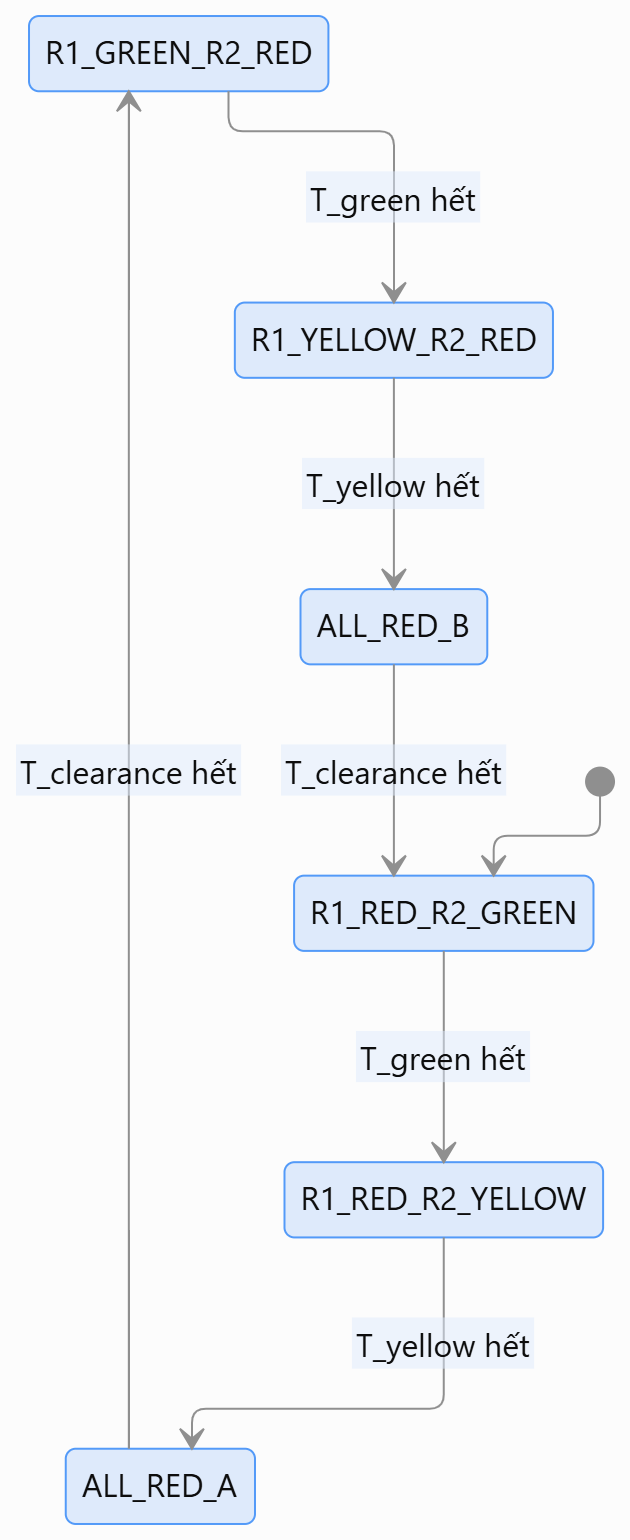
\includegraphics[width=0.92\textwidth]{graphics/fsm_automatic.png}
\caption{Sơ đồ máy trạng thái chế độ tự động (\texttt{fsm\_automatic})}
\label{fig:fsm_automatic}
\end{figure}

Bảng~\ref{tab:fsm_auto_states} mô tả chi tiết các pha hoạt động và thời lượng tương ứng:

\begin{table}[H]
\centering
\footnotesize
\begin{tabular}{|l|c|c|c|l|}
\hline
\textbf{Pha hoạt động} & \textbf{Đèn Tuyến 1} & \textbf{Đèn Tuyến 2} & \textbf{Thời lượng (s)} & \textbf{Pha kế tiếp} \\ \hline
\texttt{AUTO\_R1\_RED\_R2\_GREEN} & Đỏ & Xanh & $T_{\text{GREEN}}$ & \texttt{AUTO\_R1\_RED\_R2\_YELLOW} \\ \hline
\texttt{AUTO\_R1\_RED\_R2\_YELLOW} & Đỏ & Vàng & $T_{\text{YELLOW}}$ & \texttt{AUTO\_ALL\_RED\_AFTER\_R2} \\ \hline
\texttt{AUTO\_ALL\_RED\_AFTER\_R2} & Đỏ & Đỏ & $T_{\text{Clearance}}$ ($1\text{s}$) & \texttt{AUTO\_R1\_GREEN\_R2\_RED} \\ \hline
\texttt{AUTO\_R1\_GREEN\_R2\_RED} & Xanh & Đỏ & $T_{\text{GREEN}}$ & \texttt{AUTO\_R1\_YELLOW\_R2\_RED} \\ \hline
\texttt{AUTO\_R1\_YELLOW\_R2\_RED} & Vàng & Đỏ & $T_{\text{YELLOW}}$ & \texttt{AUTO\_ALL\_RED\_AFTER\_R1} \\ \hline
\texttt{AUTO\_ALL\_RED\_AFTER\_R1} & Đỏ & Đỏ & $T_{\text{Clearance}}$ ($1\text{s}$) & \texttt{AUTO\_R1\_RED\_R2\_GREEN} \\ \hline
\end{tabular}
\caption{Bảng trạng thái pha đèn trong chế độ tự động}
\label{tab:fsm_auto_states}
\end{table}

\subsubsection{Máy trạng thái chế độ bằng tay (\texttt{fsm\_manual})}
Khi ở chế độ bằng tay, hệ thống loại bỏ bộ đếm thời gian tự động. Các pha đèn chỉ chuyển đổi khi có sự tác động từ người điều phối thông qua Nút 2 (\texttt{FSM\_BUTTON\_ACTION}). 

\begin{figure}[H]
\centering
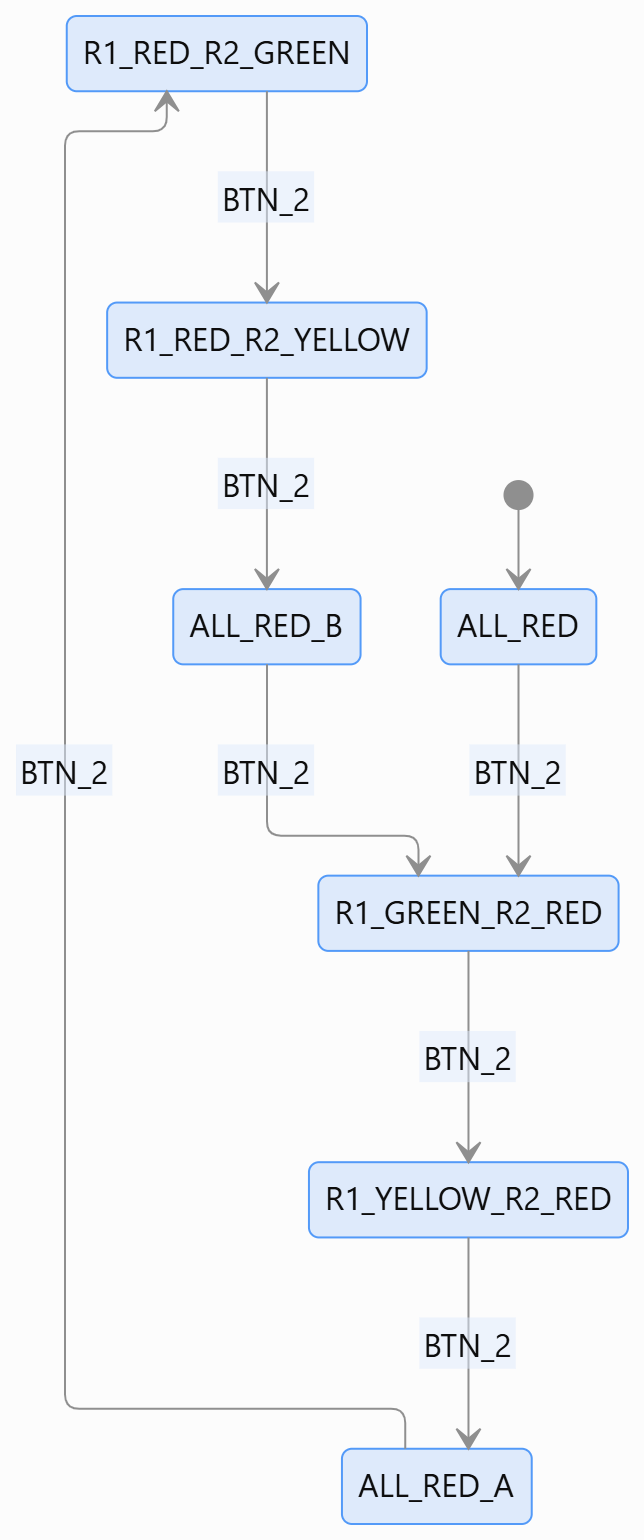
\includegraphics[width=0.88\textwidth]{graphics/fsm_manual.png}
\caption{Sơ đồ máy trạng thái chế độ bằng tay (\texttt{fsm\_manual})}
\label{fig:fsm_manual}
\end{figure}

Quy trình 7 bước tuần tự gồm:
\begin{align*}
    \text{All-Red} &\xrightarrow{\text{Nút 2}} \text{R1 Xanh, R2 Đỏ} \xrightarrow{\text{Nút 2}} \text{R1 Vàng, R2 Đỏ} \xrightarrow{\text{Nút 2}} \text{All-Red} \\
    &\xrightarrow{\text{Nút 2}} \text{R1 Đỏ, R2 Xanh} \xrightarrow{\text{Nút 2}} \text{R1 Đỏ, R2 Vàng} \xrightarrow{\text{Nút 2}} \text{All-Red}
\end{align*}
Cơ chế này đảm bảo người điều khiển bắt buộc phải kích hoạt pha All-Red trước khi mở luồng giao thông cho tuyến đối diện.

\subsubsection{Máy trạng thái chế độ chỉnh thời gian (\texttt{fsm\_tuning})}
Cho phép cấu hình các giá trị $T_{\text{RED}}$, $T_{\text{GREEN}}$, $T_{\text{YELLOW}}$ trực tiếp qua 3 nút nhấn:

\begin{figure}[H]
\centering
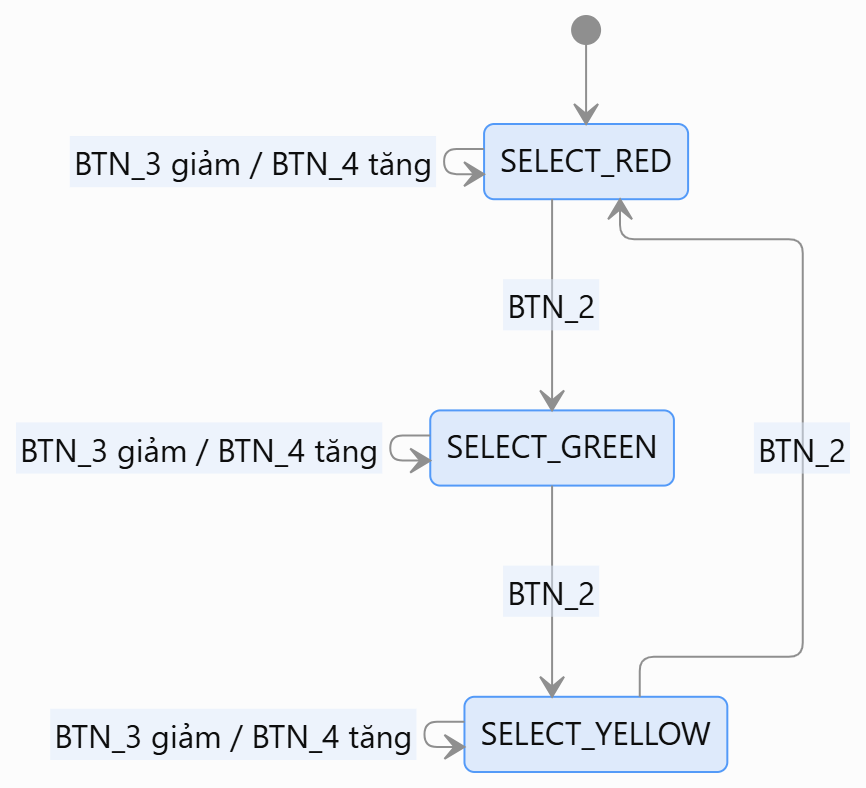
\includegraphics[width=0.85\textwidth]{graphics/fsm_tuning.png}
\caption{Sơ đồ máy trạng thái chế độ chỉnh thời gian (\texttt{fsm\_tuning})}
\label{fig:fsm_tuning}
\end{figure}

\begin{itemize}
    \item \textbf{Nút 2 (\texttt{BTN\_2})}: Chuyển đổi vòng tròn trường cần chỉnh: \texttt{TUNE\_RED} $\rightarrow$ \texttt{TUNE\_GREEN} $\rightarrow$ \texttt{TUNE\_YELLOW} $\rightarrow$ \texttt{TUNE\_RED}.
    \item \textbf{Nút 3 (\texttt{BTN\_3})}: Giảm giá trị của trường hiện tại đi 1 đơn vị.
    \item \textbf{Nút 4 (\texttt{BTN\_4})}: Tăng giá trị của trường hiện tại lên 1 đơn vị.
\end{itemize}

\subsection{Hiện thực mã nguồn máy trạng thái}
Mọi mã nguồn máy trạng thái đều tuân thủ nguyên tắc thiết kế hướng đối tượng trong C: không truy cập trực tiếp thanh ghi hay hàm HAL. Trích đoạn file \texttt{fsm\_mode\_manager.c} chứng minh việc chuyển đổi an toàn:

\begin{lstlisting}[language=C, caption={Hiện thực hàm chuyển đổi chế độ trong fsm\_mode\_manager.c}]
static void enter_mode(AppMode_t next_mode) {
    /* Cuong buc ca hai tuyen ve Den Do truoc khi sang che do moi */
    set_both_roads_red();
    setTimer(FSM_PHASE_TIMER, 0U);
    g_app_mode = next_mode;

    switch (g_app_mode) {
    case APP_MODE_AUTO:
        fsm_automatic_init();
        break;
    case APP_MODE_MANUAL:
        fsm_manual_init();
        break;
    case APP_MODE_TUNING:
        fsm_tuning_init();
        break;
    default:
        g_app_mode = APP_MODE_AUTO;
        fsm_automatic_init();
        break;
    }
}
\end{lstlisting}
Các hàm \texttt{fsm\_automatic\_run()}, \texttt{fsm\_manual\_run()} và \texttt{fsm\_tuning\_run()} chỉ được cấp quyền chạy khi biến toàn cục \texttt{g\_app\_mode} khớp với chế độ của mình, đảm bảo hệ thống độc lập và ngăn ngừa xung đột trạng thái.
